\documentclass{article}
\usepackage{graphicx} % Required for inserting images
\usepackage[a4paper, total={7in, 10in}]{geometry}
\newcommand{\forceindent}{\leavevmode{\parindent=1em\indent}}


\title{CS 440 HW2}
\author{Fulton Wilcox, Daniel Teytel, Long Tran}
\date{February 2023}

\begin{document}

\maketitle

\begin{enumerate}
\item[1:]    
Trace the operation of A∗search (use the tree version, i.e. without using a closed list) applied to the problem of getting to Bucharest from Lugoj using the straight-line distance heuristic. That is, show the sequence of nodes that the algorithm will consider and the f , g, and h score for each node. You don’t need to draw the graph, just write down a sequence of (city, f (city), g(city), h(city)) in the order in which the nodes are expanded.
\begin{enumerate}
    \item[] (Lugoj, 244, 0, 244)
    \item[] (Mehadia, 311, 70, 241)
    \item[] (Lugoj, 384, 140,244 )
    \item[] (Drobeta, 387, 145, 242)
    \item[] (Craiova, 425, 265, 160)
    \item[] (Timisoara, 440, 111, 329)
    \item[] (Mehadia, 451, 210, 241)
    \item[] (Mehadia, 456, 215, 241)
    \item[] (Lugoj, 466, 222, 244)
    \item[] (Pitesti, 503, 403, 100)
    \item[] (Bucharest, 504, 504, 0) (goal)
\end{enumerate}

\item[2:]
Consider a state space where the start state is number 1 and each state k has two successors: numbers 2k and 2k + 1.

(a) Suppose the goal state is 11. List the order in which states will be visited for breadth-first search, depth-limited search with limit 3, and iterative deepening search.

\textit{Assume for each iteration, algorithms will pick the lowest values in the available items list}

\textbf{Bread-first Search}
Pick s(1) \verb|->| expand s(2), s(3) \\
\forceindent Pick s(2) \verb|->| expand s(4), s(5) \\
\forceindent Pick s(3) \verb|->| expand s(6), s(7) \\
\forceindent\forceindent Pick s(4) \verb|->| expand s(8), s(9) \\
\forceindent\forceindent Pick s(5) \verb|->| expand s(10), s(11) \verb|->| find target 11 \verb|->| program done.\\

\textbf{Depth-limited Search with 3}

Search is limited with max depth is 3. Suppose s(1) is depth 0.

\#1 Pick s(1) \verb|->| s(2) \verb|->| s(4) \verb|->| s(8) \\
\#1.2 Pick s(1) \verb|->| s(2) \verb|->| s(4) \verb|->| s(9) \\
\#1.3 Pick s(1) \verb|->| s(2) \verb|->| s(5) \verb|->| s(10) \\
\#1.4 Pick s(1) \verb|->| s(2) \verb|->| s(5) \verb|->| s(11) \verb|->| Find target \\
\verb|->| Program done.

\textbf{Iterative Deepening Search}

\textbf{Limit = 1}\\
s(1) \verb|->| s(2)\\
s(1) \verb|->| s(3)\\
\verb|->| Reached limit


\textbf{Limit = 2}\\
s(1) \verb|->| s(2) \verb|->| s(4)\\
s(1) \verb|->| s(2) \verb|->| s(5)\\
s(1) \verb|->| s(3) \verb|->| s(6)\\
s(1) \verb|->| s(3) \verb|->| s(7)\\
\verb|->| Reached limit

\textbf{Limit = 3}\\
\#1 Pick s(1) \verb|->| s(2) \verb|->| s(4) \verb|->| s(8) \\
\#1.2 Pick s(1) \verb|->| s(2) \verb|->| s(4) \verb|->| s(9) \\
\#1.3 Pick s(1) \verb|->| s(2) \verb|->| s(5) \verb|->| s(10) \\
\#1.4 Pick s(1) \verb|->| s(2) \verb|->| s(5) \verb|->| s(11) \verb|->| Find target \\
\verb|->| Program done.

(b) How well would bidirectional search work on this problem? List the order in which states will be visited. What is the branching factor in each direction of the bidirectional search?

\textbf{Bidirectional order:}

It is sufficient to utilize bidirectional search. On the search from target, due to the node's characteristics, the branch factor (b) on the search tree from target is 1 (each number x has a parent node, which is x/2).

Therefore, each iteration on search tree from target will reduce 1 depth level for the search tree from 1.

Therefore, the time complexity reduce from $2^n$ to $2^{n/2}$

\begin{figure}[h!]
    \centering
    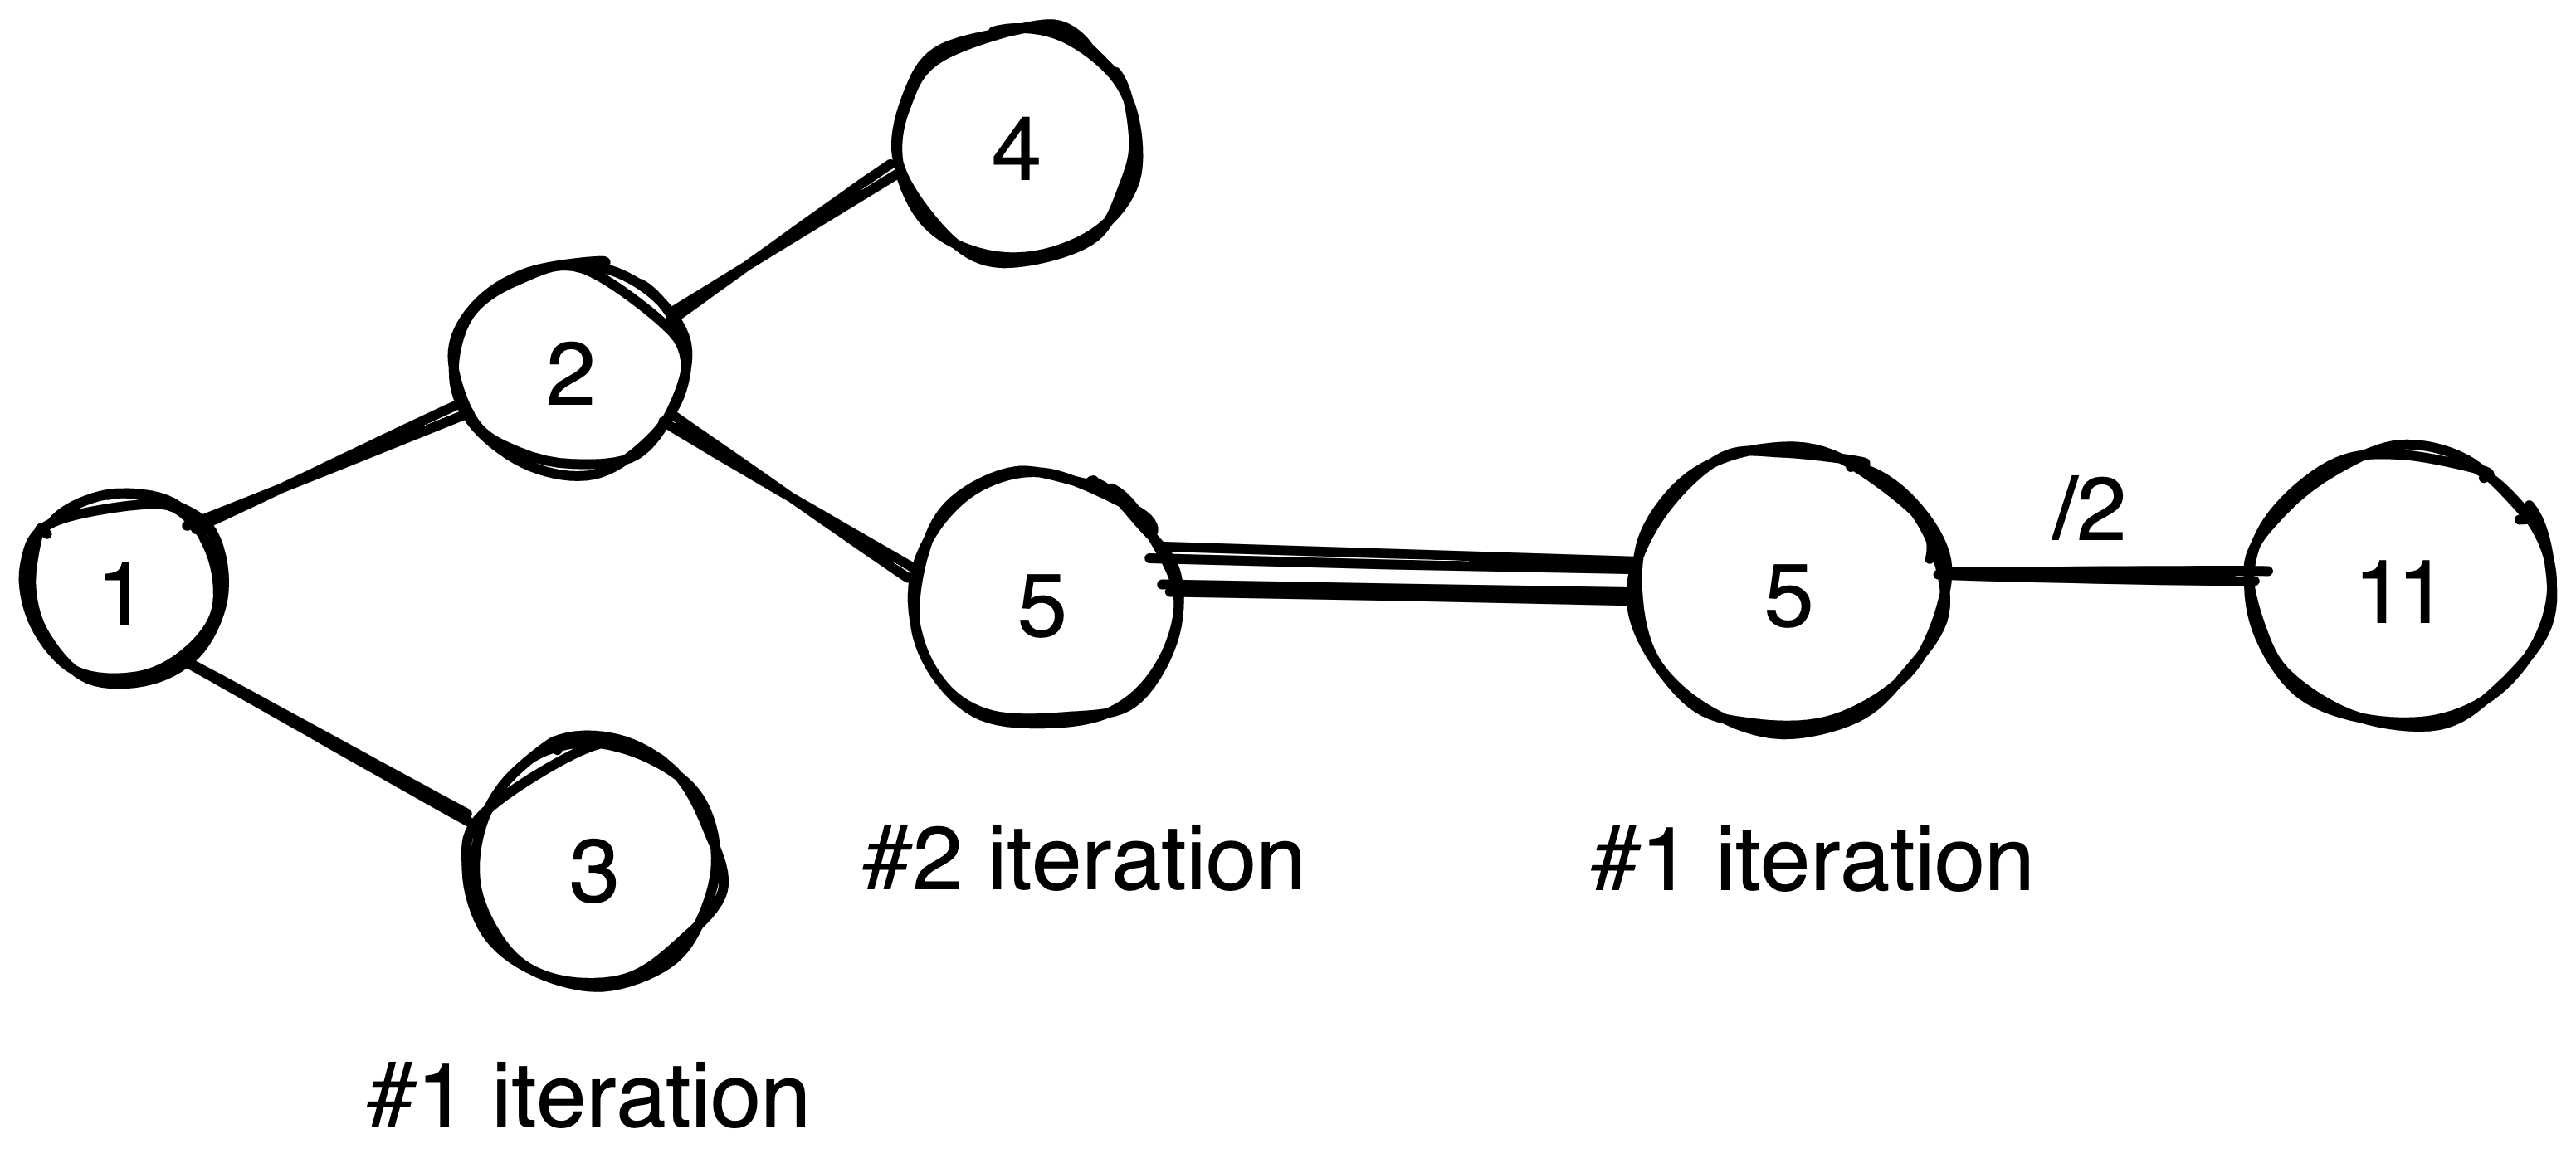
\includegraphics[width=.4\linewidth]{Hw2_2b.png}
    \caption{Bidirectional order}
    \label{bidirectional}
\end{figure}

\item[3.]
Which of the following statements are correct and which ones are wrong?

(a) Breadth-first search is a special case of uniform-cost search.

True

(b) Depth-first search is a special case of best-first tree search.

Wrong

(c) Uniform-cost search is a special case of $A\ast$ search.

True, if setting h(i) = 0 for each n.

(d) Depth-first graph search is guaranteed to return an optimal solution.

Wrong, it is bounded by max depth of the problem and may run infintely

(e) Breadth-first graph search is guaranteed to return an optimal solution.

True

(f) Uniform-cost graph search is guaranteed to return an optimal solution.

True

(g) $A\ast$ graph search is guaranteed to return an optimal solution if the heuristic is consistent.

True

(h) $A\ast$ graph search is guaranteed to expand no more nodes than depth-first graph search if the heuristic is consistent.

False, in best case, depth-first search find optimal solution in first path try.

(i) $A\ast$ graph search is guaranteed to expand no more nodes than uniform-cost graph search if the heuristic is consistent.

True

\item[4.]
Iterative deepening is sometimes used as an alternative to breadth first search. Give one advantage
of iterative deepening over BFS, and give one disadvantage of iterative deepening as compared with BFS. Be concise and
specific

\textbf{Advantage of Iterative Deepening}\\
- Due to the utilization of recursion function, it consumes much less memory.
Suppose search tree has large branching factor (b) and current depth limit is d, the memory it uses is to memorize the current path and the b branches at d level.
\verb|->| It consumes d + b of memory space.
Meanwhile, BFS consumes $b^d$ of memory space to memorize all the states.

\verb|->| Iterative Deepening Search has much more efficient space complexity.

\textbf{Disadvantage of Iterative Deepening}
- It revisits the states many time. Each time it increases the depth limit, it would revisit the start states again.\\
- If a target is found at depth d and tree search has branch factor b, the total number of search revisits each depth i is 
\[ \Sigma_{i=0}^d (d-i+1) \ast b^i \]
\[ b^d \ast (1 - 1/b)^{-2} \]
\[ = O(b^d)\]

Comparing to BFS, Iterative Deepening has same Time Complexity but its cons is to revisiting states as a constant rate.

\item[5.]
Prove that if a heuristic is consistent, it must be admissible. Construct an example of an admissible
heuristic that is not consistent. (Hint: you can draw a small graph of 3 nodes and write arbitrary cost and heuristic values
so that the heuristic is admissible but not consistent).

(Assuming the minimum cost between nodes is $>$ 0)\\
Consider any arbitrary graph G and a path P consisting of 3 nodes \{n, n', target node\}.  Also assume n and target node are connected.  Under the assumption of consistency, h(n) is bounded above by h(n') + g(n) where g(n) is the step cost from n to n'.  The true cost from n to the target node is g(n) + g(n').  Given that n' and the target node are connected, h(n') = g(n').  The upper bound for h(n) can then be expressed as g(n) + g(n'), which is the true cost from n to target.  If h(n) exceeded this, it would be an overestimation of the true cost from n to target, which contradicts admissibility.  As a result, all consistent heuristics must be admissible.

\begin{figure}[h!]
    \centering
    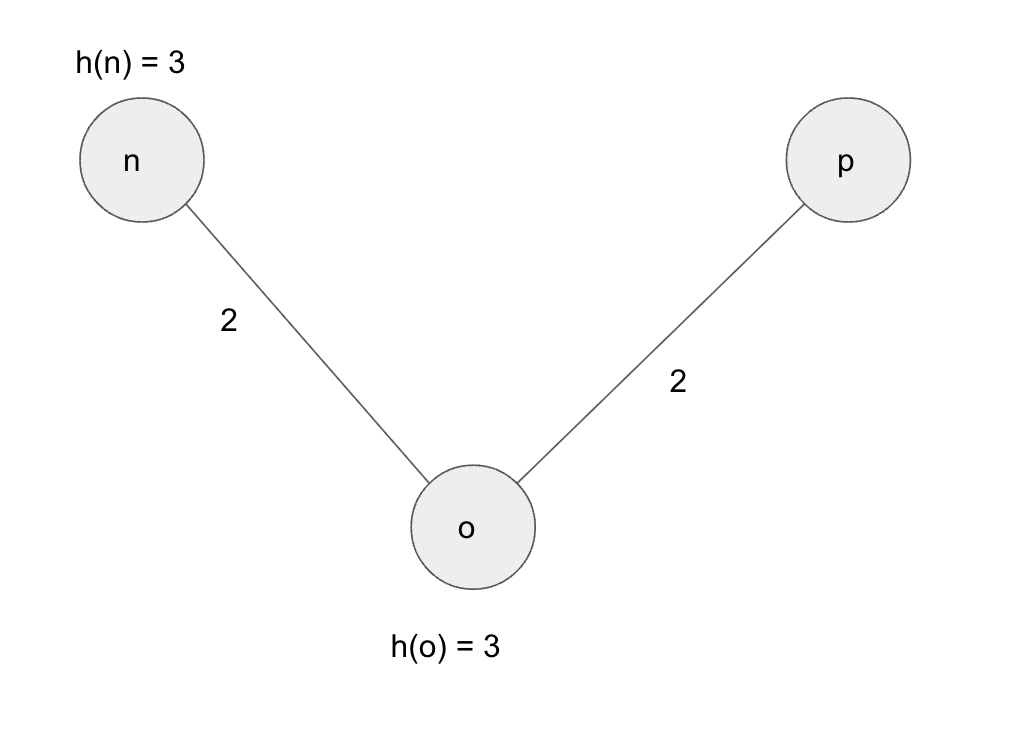
\includegraphics[width=.4\linewidth]{graph.png}
    \caption{}
    \label{bidirectional}
\end{figure}

This heuristic is admissible because for n and o (where p is the target), h(n) and h(o) underestimate the true costs for n and o, respectively.  However, h(o) $>$ g(o, p, op) + h(p).

\item[6.] In any constraint satisfaction problem, it is a good idea to select the variable that is the most constrained because there will be less wasted time pruning a corresponding branch that will fail because a variable with more constraints is likely to fail earlier than a less constrained variable.  Choosing the value that's the least constrained is also a good idea because it rules out fewer options for neighboring variables. 

\end{enumerate}


\end{document}
